% Vorlage für ein Ofahrtheft
% Erstellt von: Tobias Otterbein, totterbein@d120.de, Stand: 02.11.2017
% Editiert von der Leitung 2017
% Darf beliebig angepasst werden.
\documentclass[a5paper,pagesize,twoside,fontsize=8pt,DIV=15]{scrreprt}

\usepackage{ofahrtheft}

% Sprache hier einstellen
\usepackage[ngerman]{babel}
\usepackage[utf8]{inputenc}
\usepackage{marvosym}
\usepackage{blindtext}


% \workshop
% 1: Titel
% 2: Anbietende Personen
% 3: Zeitslots
% 4: Beschreibungstext
% 5: Maximale Teilnehmer*innenzahl
% 6: Benötigtes Material
% 7: Voraussetzungen zur Teilnahme
% 8: Sonstige Infos


\begin{document}

% Titelseite
\begin{titlepage}~


\begin{textblock*}{5cm}(8cm,1.5cm)

\includegraphics[width=5cm]{logo_ohne_rand}
\end{textblock*}


\begin{textblock*}{12cm}(2.5cm,6cm)
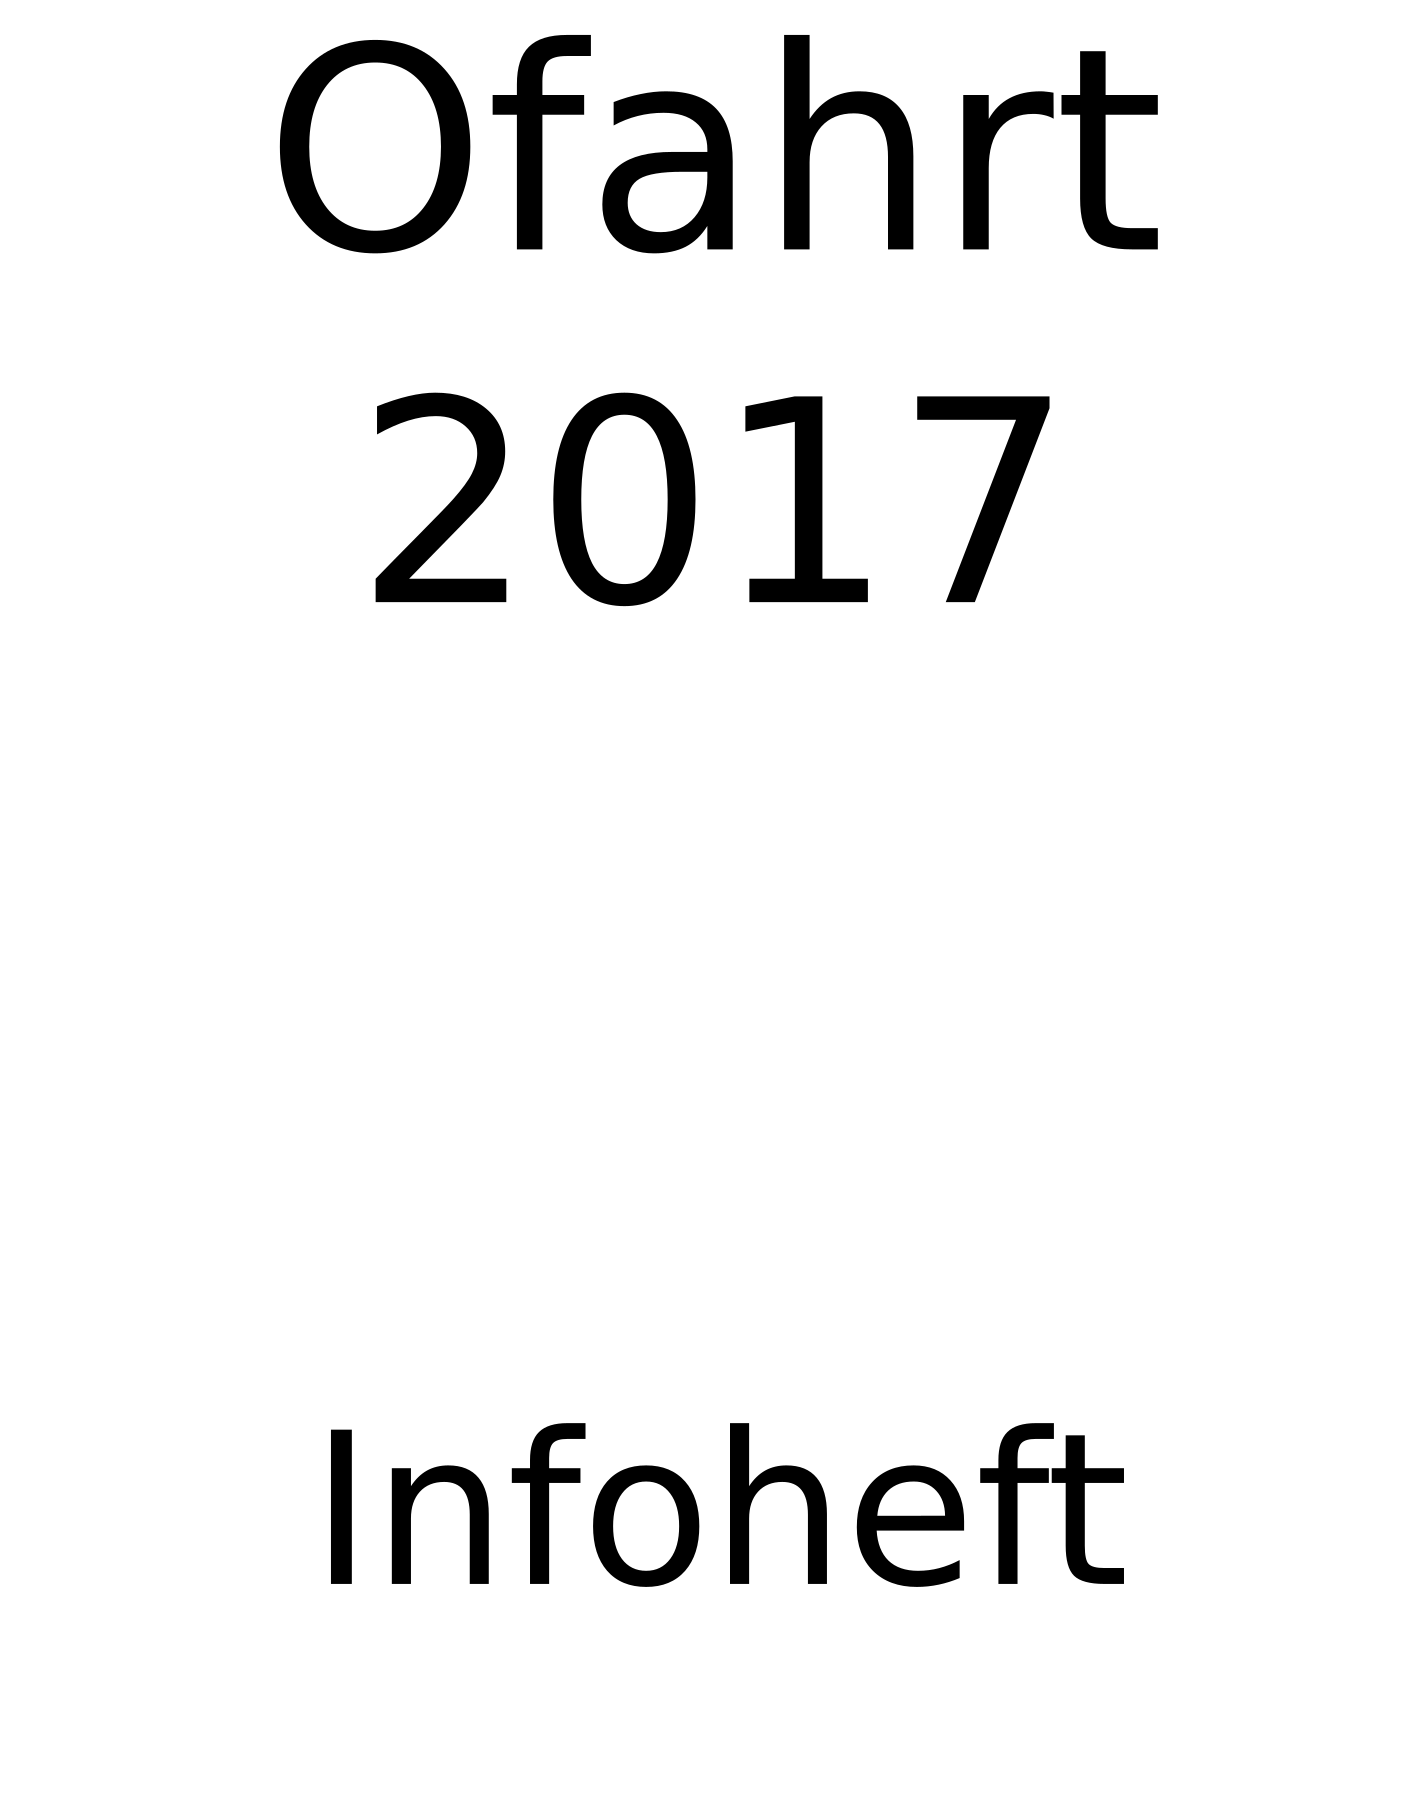
\includegraphics[width=10cm]{titel}
\end{textblock*}






\end{titlepage}
\newpage

% Vorwort
\addsec{Liebe Teilnehmer*innen der Ofahrt,}

Herzlich Willkommen auf der diesjährigen Ofahrt.

\vspace{3mm}

Dieses Heft soll euch eine Übersicht über alle wichtigen Infos und den Workshops auf der Ofahrt bieten. Die hier enthaltenen Infos erhaltet ihr ebenfalls während des Anfangsplenums. \textbf{Bitte nutzt dieses Heft daher als Nachschlagewerk und nicht während des Plenums ;-)}. 

\vspace{3mm}

Wir veranstalten die Ofahrt dieses Jahr zum allerersten Mal, daher könnte es sein, dass nicht alles perfekt läuft. Wir freuen uns daher über Kritik und Anregungen, um in den nächsten Jahren die Ofahrt besser zu machen. Die Orgas und Workshopanbieter*innen erkennt ihr an den grünen Namensschildern.

\vspace{3mm}

Wir alle sind hier zu Gast auf der Starkenburg und möchten euch daher bitten, euch entsprechend der von den "`Burgherren"' (also der Jugendherbergsleitung) aufgestellten Regeln zu verhalten. 

\vspace{3mm}

Wir wünschen euch in den drei Tagen hier auf der Burg viel Spaß und hoffen, dass ihr auch einige neue Leute kennenlernen könnt.

\vspace{5mm}

Die Ofahrt-Orga


\newpage


% Inhalt

\kapitel{Wichtige Infos}{}{Organisatorisches und Regeln}{}

\addsec{Ablauf}
Einen detaillierten Ablaufplan findest du auf der Rückseite dieses Hefts. Wir unterscheiden zwischen Gemeinschafts- und Kleingruppen-Veranstaltungen.

\vspace{-2mm}

\addsec{Essen}
Feste Essenszeiten gemeinsam im großen Speisesaal:
\begin{itemize}
\item Frühstück: 08:15 bis 09:15
\item Mittagessen: 12:00 bis 13:00
\item Abendessen: 18:00 bis 19:00
\end{itemize}


Abseits dieser Zeiten stehen Tee/Wasser frei zur Verfügung, wahlweise auch mit Kohlensäure. Snacks und weitere Getränke werden von uns zum Selbstkostenpreis angeboten, was über eine Kasse des Vertrauens (KdV) funktioniert, die weiter unten nochmal genau erklärt ist. Alkoholische Getränke über 10 Vol.\% werden wir nicht von uns aus anbieten. Außerdem ist vor Ort ein Snack-Automat verfügbar.


\subsection*{Kasse des Vertrauens (KdV)}

Bei der KdV ist jede*r Käufer*in für die korrekte Begleichung des Betrags selbst verantwortlich. Wir vertrauen darauf, dass ihr alle Snacks und Getränke gewissenhaft abscannt, damit wir nicht auf den Unkosten sitzen bleiben.\\

\textbf{KdV-Bedienung:}
\begin{enumerate}
    \item Eigenen Barcode scannen (Rückseite des Namensschildes)
    \item Die KdV zeigt aktuellen Stand des eigenen Kontos an
    \item Artikel scannen
    \item Artikel wird direkt gebucht 
    \item Eigenes Konto ausloggen (Barcode an dem Gerät)
    \item Fertig
\end{enumerate}

\textbf{Die Anzeige der KdV:}
\begin{itemize}
    \item Oben Links: Accountname
    \item Oben Rechts: Aktueller Betrag (nach Kauf/Storno)
    \item Mitte Links: Gescanntes Produkt
    \item Unten Links: Preis des Produkts
\end{itemize}

\textbf{Widerruf der letzten Transaktion:}
\begin{enumerate}
    \item Eigenen Barcode scannen
    \item Storno-Code scannen (befindet sich auf KdV)
    \item letzte Transaktion wird storniert
\end{enumerate}
Damit lassen sich auch mehr als eine Transaktion stornieren.
Bei Fragen einfach an die Orgas wenden, wir helfen euch gerne.
\textbf{Vor Abreise (oder auch schon zwischendurch): Rechnung begleichen.}

\newpage

\addsec{Orientierung}

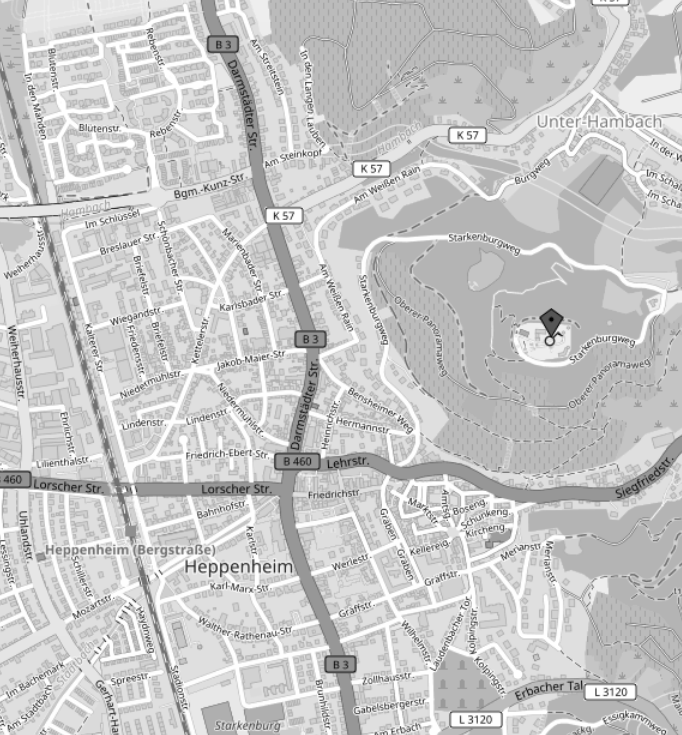
\includegraphics[width=\textwidth]{umgebung_big}

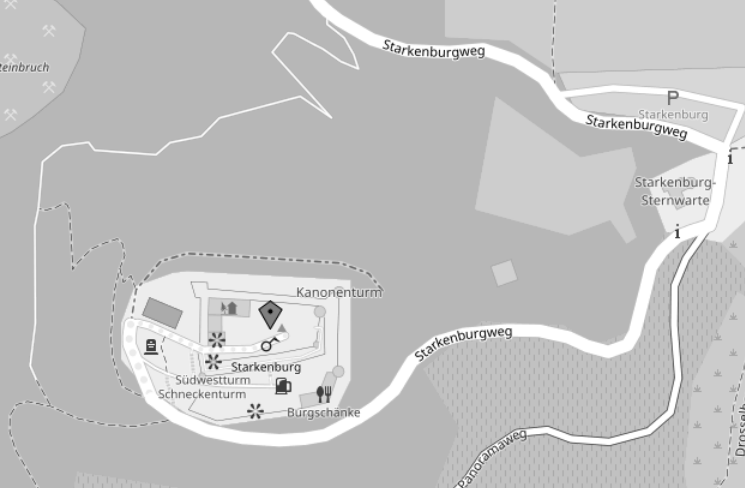
\includegraphics[width=\textwidth]{umgebung_small}

\newpage

\addsec{Freizeitaktivitäten und Workshops}
Wir bieten neben den Workshops in Kleingruppen auch gemeinsame Freizeitaktivitäten an. Dazu gehören die folgenden Punkte.

\subsection*{Nachtwanderung \& Lagerfeuer}
Bei der Nachtwanderung werden wir die waldige Umgebung der Starkenburg erkunden, zum Abschluss wird ein Lagerfeuer entfacht - natürlich mit Stockbrot und Marshmallows!

\subsection*{Party}
Ich sag Disko, du sagst Party! Disko Disko! .... Party? Party!

\subsection*{Workshops}
In den Workshops werden, in Anlehnung an die Ophase, einerseits Einblicke in interessante Themen des Universitätslebens und der Informatik geboten, andererseits auch aktive Programmpunkte zum Auspowern angeboten. Die Anzahl der Teilnehmenden für die Workshops ist begrenzt, der genaue Ablauf der Anmeldung wird im Anfangsplenum erläutert.
Auf den folgenden Seiten werden die einzelnen Workshops mit Voraussetzungen vorgestellt.

\addsec{Abreise}
Leider hat auch die Ofahrt ein Ende. Ab Sonntag, 14:00 Uhr ist alles vorbei und ihr werdet die Ofahrt hoffentlich in toller Erinnerung behalten! :-)
Damit alles reibungslos abläuft, gibt es allerdings noch zwei kleine Auflagen, die ihr wahrscheinlich schon von anderen Herbergsbesuchen kennt und immer eingehalten werden müssen.

\begin{itemize}
    \item Zimmerräumung bis um 10:00 Uhr. Das Gepäck kann bis zur Abreise in einem Gepäckraum gelagert werden.
    \item Ein guter Gast hinterlässt ein Zimmer so, dass man gar nicht erkennen kann, dass dort gehaust wurde. Bitte lasst also das Zimmer in dem Zustand zurück, in dem ihr es vorgefunden habt.

\end{itemize}


Vielen Dank!
Eure Ofahrt-Orga



\kapitel{Workshops}{}{Viele bunte Workshops}{}



%\workshop{Einführung in \LaTeX}{Tobias Otterbein}{Slot 1}{\blindtext[2]}{15 Teilnehmer*innen}{Laptop}{Installiertes TeX}{Ähnlich zum Ophasenworkshop. Weiterführendes im nächsten Slot}{Raum A}
%\workshop{Ein weiterer toller Workshop mit \LaTeX}{Tobias Otterbein}{Slot 2}{\blindtext[2]}{15 Teilnehmer*innen}{Laptop}{Installiertes TeX}{Ähnlich zum Ophasenworkshop. Weiterführendes im nächsten Slot}{Raum B}

\workshop{{workshop.name|tex_escape}} }{ {{host.get_full_name}},  }{ {{workshop.slot}} }{ {{workshop.description|tex_escape}} }{ {{workshop.maxmembers|tex_escape}} }{ {{workshop.requirements|tex_escape}} }{ {{workshop.conditions|tex_escape}} }{ {{workshop.otherstuff|tex_escape}} }{ {{workshop.room}} }





\notizen





\newpage
% Rückseite

%\ThisCenterWallPaper{1}{grafik/Plakat1400}

\thispagestyle{empty}
\addsec{Stundenplan}
%\renewcommand{\arraystretch}{5.5}
\begin{tabular}{|c|c|c|c|c|}
\hline
\multirow{3}{*}{\textbf{Zeit}} & \multirow{3}{*}{\textbf{Freitag}} &\multicolumn{2}{c|}{\multirow{3}{*}{\textbf{Samstag}}} & \multirow{3}{*}{\textbf{Sonntag}}\\
& & \multicolumn{2}{c|}{} & \\
& & \multicolumn{2}{c|}{} & \\
\hline
\multirow{3}{*}{08:30 - 09:30} & & \multicolumn{2}{c|}{\multirow{3}{*}{Frühstück}} & \multirow{3}{*}{Frühstück}\\
& & \multicolumn{2}{c|}{} & \\
& & \multicolumn{2}{c|}{} & \\
\cline{1-1}\cline{3-5}
\multirow{6}{*}{09:30 - 12:00} &  &\multicolumn{2}{c|}{} & \\
& & \multicolumn{2}{c|}{1. Gruppenphase} & 5. Gruppenphase \\
& & \multicolumn{2}{c|}{} & \\
& &  \multicolumn{2}{c|}{} & \\
& &  \multicolumn{2}{c|}{} & \\
& & \multicolumn{2}{r|}{\WritingHand}&  \multicolumn{1}{r|}{\WritingHand}\\
\cline{1-1}\cline{3-5}
\multirow{3}{*}{12:30 - 13:30} & & \multicolumn{2}{c|}{\multirow{3}{*}{Mittagessen}} & \multirow{3}{*}{Mittagessen}\\
& & \multicolumn{2}{c|}{}& \\
& & \multicolumn{2}{c|}{}& \\
\cline{1-1}\cline{3-5}
\multirow{6}{*}{14:00 - 16:30} & &  \multicolumn{2}{c|}{} & \\
& & \multicolumn{2}{c|}{2. Gruppenphase} & Abreise \\
& & \multicolumn{2}{c|}{} & \\
\cline{5-5}
& &  \multicolumn{2}{c|}{} & \\
& &  \multicolumn{2}{c|}{} &\\
& & \multicolumn{2}{r|}{\WritingHand} & \\
\cline{1-4}
\multirow{6}{*}{16:30 - 19:00} & \multirow{5}{*}{Anfangsplenum} &   \multicolumn{2}{c|}{} & \\
& & \multicolumn{2}{c|}{3. Gruppenphase} & \\
& & \multicolumn{2}{c|}{}& \\
& &  \multicolumn{2}{c|}{} & \\
& &  \multicolumn{2}{c|}{} &\\
\cline{2-2}
& &  \multicolumn{2}{r|}{\WritingHand} & \\
\cline{1-4}
\multirow{3}{*}{19:00 - 20:00} & \multirow{3}{*}{Abendessen} & \multicolumn{2}{c|}{\multirow{3}{*}{Abendessen}} & \\
& & \multicolumn{2}{c|}{}& \\
& & \multicolumn{2}{c|}{}& \\
\cline{1-4}
\multirow{2}{*}{20:00} & \multirow{4}{*}{Nachtwanderung} & \multicolumn{2}{c|}{\multirow{2}{*}{}}  &\\
& &  \multicolumn{2}{c|}{} & \\
\cline{1-1}\cline{3-3}
\multirow{2}{*}{20:30} &  & \multirow{2}{*}{4. Gruppenphase} & & \\
&  &  & & \\
\cline{1-2}\cline{4-4}
\multirow{4}{*}{21:00} &\multirow{4}{*}{Lagerfeuer} & (bis 22:30) &\multirow{4}{*}{Party} & \\
& &  & & \\
& &  & & \\
& &  \multicolumn{1}{r|}{\WritingHand} & & \\
\hline


\end{tabular}

\vspace{3mm}
\WritingHand : Deine Workshops kannst du hier eintragen.

\end{document}
